\setlength{\droptitle}{-4\baselineskip} % Move the title up
\pretitle{\begin{center}\Huge\bfseries} % Article title formatting
    \posttitle{\end{center}} % Article title closing formatting
\title{VA - Roman Empire} % Article title
\author{
  \textsc{Luigi Russo, Matteo Salvino}\\[1ex] % Authors
  \normalsize Sapienza University of Rome \\ % Your institution
}
\date{\today} % Leave empty to omit a date

\renewcommand{\maketitlehookd}{
  \begin{minipage}{\linewidth}
    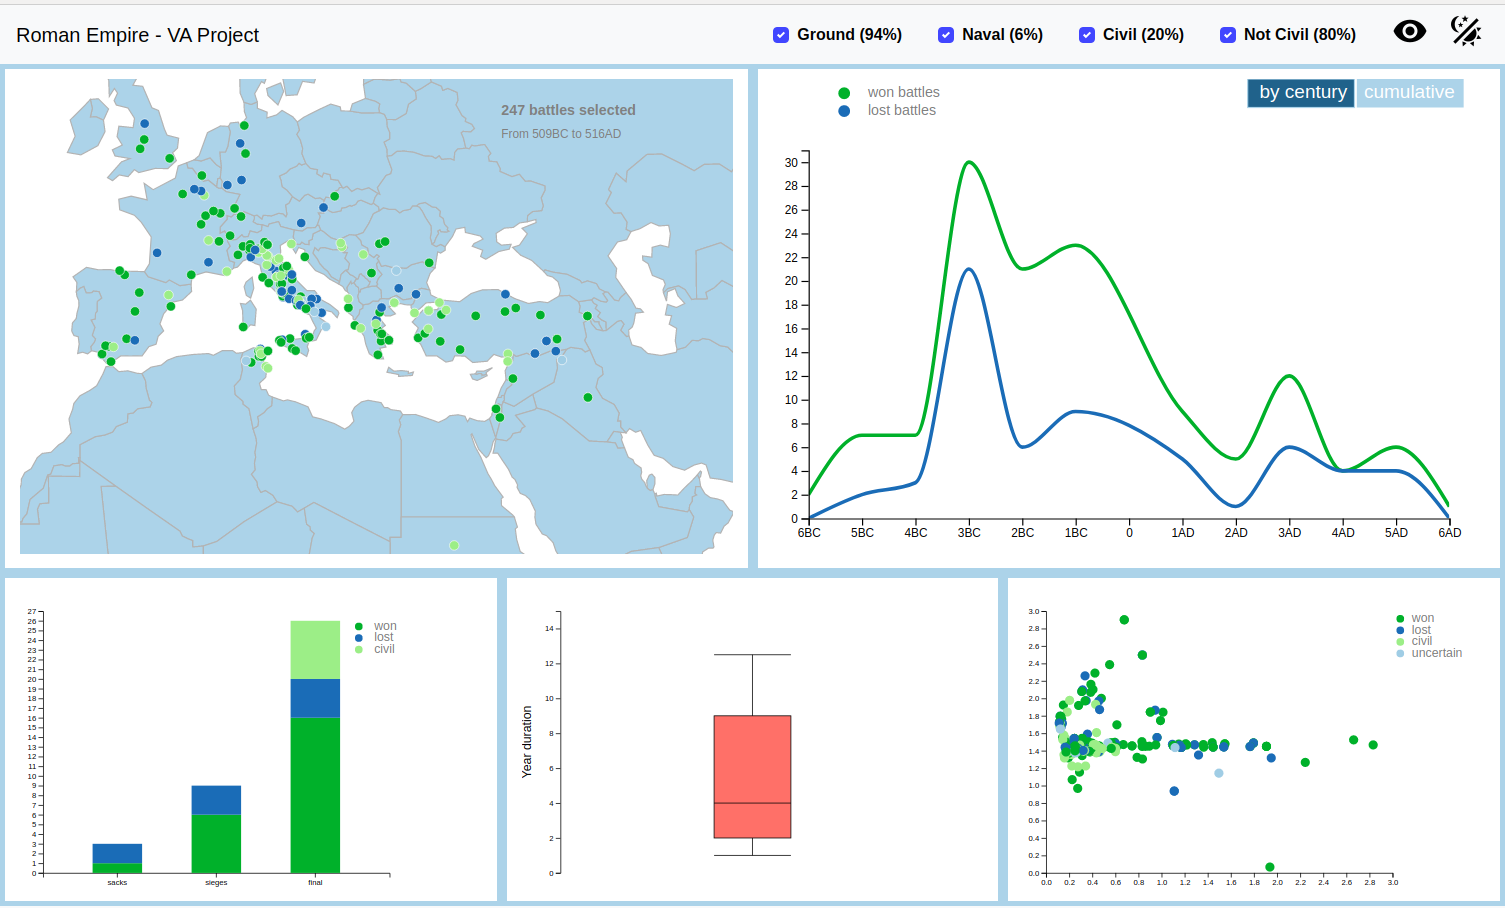
\includegraphics[width=\linewidth]{./images/visualization_views.png}
    \captionof{figure}{Visualization with light mode enabled and blind safe mode disabled}
  \end{minipage}

  \begin{abstract}
    \noindent The military of ancient Rome is unanimously considered a key element in the rise of Rome and for this reason we developed a visual analytics tool to help users to learn the battles details that this empire has faced. The multiple interactive views of our project present high level features, but the user has also the possibility to explore further information via the reference link of a specific battle.
  \end{abstract}
}